\documentclass[areasetadvanced]{scrartcl}

\usepackage[utf8]{inputenc}
\usepackage[T2A]{fontenc}
\usepackage[english,russian]{babel}
\usepackage{xcolor}
\usepackage{ulem}

% Добавляем пакеты для математических операторов
\usepackage{amsmath}
\usepackage{amssymb}
\usepackage{amsthm}
\usepackage{mathrsfs}

% Определяем недостающие операторы
\DeclareMathOperator{\Dom}{Dom}
\DeclareMathOperator{\E}{E}
\DeclareMathOperator{\Lap}{Lap}

% Заменяем устаревшие команды
\newcommand{\rmtot}{\mathrm{tot}}
\newcommand{\rmavg}{\mathrm{avg}}

\usepackage[footskip=1cm,left=25mm, right=15mm, top=20mm, bottom=20mm]{geometry}
\usepackage{setspace}
\usepackage{amsmath, amssymb} 
\usepackage{graphicx}
\usepackage{tikz}
\usetikzlibrary{arrows.meta}
\usepackage{float}
\usepackage{dashrule}
\usepackage{fancyhdr} 
\usepackage{hyperref} 
\usepackage{parskip}
\usepackage{textcomp, enumitem}
\usepackage{indentfirst}
\usepackage{graphicx}
\usepackage{algorithm}
\usepackage{algpseudocode}
\usepackage{array} 
\usepackage{geometry}
\usepackage{afterpage}
\usepackage{minted}
\setcounter{secnumdepth}{3} 
\setcounter{tocdepth}{3}    
\usepackage{listings} 

\tikzstyle{block} = [rectangle, rounded corners, minimum width=3cm, minimum height=1cm, text centered, draw=black, fill=lightgray]

\setkomafont{sectioning}{\normalfont\bfseries} 
\setkomafont{section}{\normalfont\Large\bfseries}
\setkomafont{subsection}{\normalfont\large\bfseries}
\setkomafont{subsubsection}{\normalfont\large\bfseries}
\setkomafont{paragraph}{\normalfont\large\bfseries} 

\lstset{
  language=Haskell,
  basicstyle=\ttfamily\small,
  keywordstyle=\color{blue}\bfseries,
  stringstyle=\color{red},
  commentstyle=\color{green!70!black},
  numbers=left,
  numberstyle=\tiny,
  stepnumber=1,
  numbersep=10pt,
  showstringspaces=false,
  breaklines=true,
  frame=single
}

\setcounter{tocdepth}{2}
\begin{document}
\sloppy
	\thispagestyle{empty}
	\begin{center}
		\large{МИНОБРНАУКИ РОССИИ} \par
		\vspace{0.3cm}
		\normalsize
		{ФЕДЕРАЛЬНОЕ ГОСУДАРСТВЕННОЕ АВТОНОМНОЕ ОБРАЗОВАТЕЛЬНОЕ УЧРЕЖДЕНИЕ ВЫСШЕГО ОБРАЗОВАНИЯ} \par
		\vspace{0.3cm}
		\textbf{\guillemotleft САНКТ-ПЕТЕРБУРГСКИЙ ПОЛИТЕХНИЧЕСКИЙ}
		\textbf{УНИВЕРСИТЕТ ПЕТРА ВЕЛИКОГО\guillemotright} \par
		\vspace{0.3cm}
		{Институт компьютерных наук и кибербезопасности}\par
		{Высшая школа технологий искусственного интеллекта}\par
	\end{center}
	\vfill
	\begin{center}
		{\large Отчёт по дисциплине \guillemotleft Образовательный форсайт\guillemotright}\par
		{\huge   Анонимизация данных}\par 
         
	\end{center}
	\vfill
	\begin{flushleft}
		Студент: \hspace{1.8cm} \rule[0pt]{2.5cm}{0.5pt}\hfill Салимли Айзек Мухтар Оглы\par
		\vspace{1.5cm}
		Преподаватель: \hspace{0.55cm} \rule[0pt]{2.5cm}{0.5pt}\hfill  Курочкин Михаил Александрович
	\end{flushleft}
	\vspace{0.5cm}
	\begin{flushright}
		\guillemotleft \rule[0pt]{0.8cm}{0.5pt}\guillemotright \rule[0pt]{2cm}{0.5pt} 20\rule[0pt]{0.5cm}{0.5pt} г.
	\end{flushright}
	\vfill
	\begin{center}
		Санкт-Петербург, 2025
	\end{center}
	\newpage
	\tableofcontents
	\newpage
\section*{Введение}
	\addcontentsline{toc}{section}{Введение}
    В рамках модуля мобильности был выбран курс «Анонимизация данных», так как направление данного курса, нужно для защиты персональных данных.
    Автором курса, является ведущий специалист в области анонимизации данных - д.т.н., доцент Института компьютерных наук и кибербезопасности - Полтавцева Мария Анатольевна.
    Курс включает в себя 6 содержательных тем. Все материалы курса доступны с
    момента открытия курса: видеолекции, кратко раскрывающие содержание каждой темы,
    презентации и конспекты, с которыми в дальнейшем можно ознакомиться в любое удобное
    время. Все темы включают практические занятия и самостоятельные работы. В материалах
    курса подготовлены методические рекомендации к выполнению заданий и примеры решения
    типовых заданий.

\newpage
\section{Постановка задачи}
В рамках курса «Образовательный форсайт», было необходимо пройти выбранный по желанию
онлайн курс «Анонимизация данных» на портале «Открытое
образование» (https://openedu.ru/).
Онлайн-курс предполагает успешное освоение предлагаемых десяти лекций, написание
контрольных заданий по лекциям и итогового теста.
Цель изучения дисциплины «Анонимизация данных»
заключается в освоении базовых принципов и методов анонимизации данных.

\newpage
\section{Аннотация курса и разделов}
В настоящее время анонимизация данных является критически важным направлением в области информационной безопасности и защиты персональных данных. 
Этот курс представляет собой комплексное изучение современных методов и технологий обеспечения конфиденциальности информации в условиях цифровой трансформации. 
Анонимизация данных формирует основу для безопасной работы с персональной информацией, 
позволяя использовать данные для анализа и исследований, сохраняя при этом приватность пользователей.

Технологии анонимизации находят широкое применение в различных сферах деятельности, включая здравоохранение, финансы, государственное управление и бизнес-аналитику. 
Они предоставляют возможность работать с большими объемами данных, соблюдая требования законодательства о защите персональных данных и 
обеспечивая баланс между доступностью информации и её конфиденциальностью. 
Это делает знания в области анонимизации данных особенно ценными в современном мире, где вопросы защиты информации становятся все более актуальными.

\newpage
\section{Теоретическая часть курса}
\subsection{Базовые понятия}
\begin{itemize}
    \item \textbf{Анонимизация (персональных) данных} - действия, направленные на сохранение конфиденциальности данных путем защиты от атак идентификации.
    
    \item \textbf{Атака логического вывода (inference attack)} – атаки нарушения конфиденциальности данных, которые проводятся без нарушения политики безопасности, как правило, с использование внешних знаний и данных.
    
    \item \textbf{Атаки идентификации} – вид атак логического вывода, которые позволяют в наборе данных (в том числе, обезличенном, из которого удалена персональная информация) установить кортежи, или сведения, принадлежащие конкретному субъекту.
    
    \item \textbf{Обезличивание (персональных) данных} - действия, в результате которых становится невозможным без использования дополнительной информации определить принадлежность персональных данных конкретному субъекту персональных данных.
    
    \item \textbf{Обратная идентификация} - установление по защищенным данным сведений, относящихся к конкретному лицу (объекту) путем восстановления исходных данных на основе только обезличенного набора.
    
    \item \textbf{Повторная идентификация} - установление по защищенным (обезличенным или анонимизированным) данным сведений, относящихся к конкретному лицу (объекту).
    
    \item \textbf{Повторная идентификация с использованием фоновых знаний} - установление по защищенным данным сведений, относящихся к конкретному лицу (объекту) путем восстановления исходных данных с использованием внешних знаний и/или данных.
\end{itemize}
% Предполагается, что этот фрагмент включается в тело LaTeX-документа

\subsection{Атаки идентификации и анонимизация данных}

\paragraph{Логический вывод и атаки идентификации.}  
Атаки логического вывода (inference attacks) не нарушают политику доступа, но с помощью доступных агрегированных данных и фоновых знаний позволяют вывести конфиденциальную информацию о конкретном субъекте.

\paragraph{Повторная идентификация.}  
\begin{itemize}
  \item \emph{Обратная идентификация:} восстановление исходных данных $X$ по обезличенному $X'$ и знанию алгоритма $f$, $X = f^{-1}(X')$.
  \item \emph{С фоновыми знаниями:} объединение обезличенных данных $X'$ с внешними источниками $B$ для установления соответствия.
\end{itemize}

\paragraph{Законодательные требования.}  
Федеральный закон~152-ФЗ:
\[
  \text{обезличивание}~X:\quad
  \nexists\;\text{доп. инфо.}\;\Rightarrow
  \neg\bigl(\text{определить субъекта по }X\bigr).
\]
Приказ РКН~№996 выделяет четыре подхода к обезличиванию:
\begin{enumerate}
  \item введение идентификаторов;
  \item изменение состава и семантики данных;
  \item декомпозиция;
  \item перемешивание.
\end{enumerate}

\subsection{Методы обезличивания данных}

\paragraph{Требования к методам.}  
Методы должны обеспечивать:
\begin{enumerate}
  \item \emph{Невозможность восстановления} исходных $X$ из $X'$: $\nexists\,f^{-1}$;
  \item \emph{Сохранение домена и формата:} $X'_i\in\Dom(X_i)$;
  \item \emph{Уникальность:} если $X_i\neq X_j$, то $X'_i\neq X'_j$;
  \item \emph{Ссылочная целостность} при нескольких таблицах;
  \item \emph{Применимость ко всем значениям} домена;
  \item \emph{Сохранение статистик:} оценки по агрегатам должны быть близки.
\end{enumerate}

\paragraph{Обратимые методы.}
\begin{itemize}
  \item \textbf{Декомпозиция}: разделение на таблицы $T_1(ID,\dots), T_2(ID,\dots)$ по суррогатному ключу~$ID$.
  \item \textbf{Подстановка}: $x_i \mapsto t(x_i)$, где $t$ задано таблицей соответствий.
  \item \textbf{Преобразование}: 
    \[
      V_d = F(V_u, V_r),\quad
      V_u = F^{-1}(V_d, V_r).
    \]
  \item \textbf{Перестановка}: обмен полями между записями; если алгоритм детерминирован, — обратимо.
\end{itemize}

\paragraph{Необратимые методы.}
\begin{itemize}
  \item \textbf{Замена на константу:} $x_i\to*$.
  \item \textbf{Округление:} $x_i\to b\left\lfloor x_i/b\right\rceil$, риск раскрытия
    \(\displaystyle DR(X[i])=\frac1{\log_2 m(I[i])}\).
  \item \textbf{Микроагрегация:} группы размера $\ge k$, замена на среднее. Риск
    \(\displaystyle DR_w=\frac1n\sum_{k,j}w_{kj}c_{kj}.\)
  \item \textbf{Обобщение:} замена конкретных значений на более общие (даты → месяцы).
  \item \textbf{Размытие (blurring):} $x_i\to x_i+\eta$, $\eta$ случайно в малом диапазоне.
\end{itemize}

\subsection{Концепция предположительной анонимности}

\paragraph{Модель угадывания.}  
Пусть $I\in\{1,\dots,M\}$ — индекс записи с псевдоидентификатором $r_i$, а $S$ — наблюдаемый шумом выход.  
Число догадок $G(I|s)$ оптимальной стратегии минимизирует $\E[G(I|S)]$.

\paragraph{Границы по энтропии Реньи.}  
\[
  \E\bigl[G(I|S)\bigr]^\rho \;\le\; H_\alpha(I|S),
\]
где
\(
  H_\alpha(I|S)
  = \frac1{1-\alpha}\ln \sum_s \sum_i P(i,s)^\alpha.
\)

\paragraph{Gaussian-модель.}  
При $S\mid I=i\sim\mathcal N(r_i,\sigma^2)$ нижняя граница
\[
  \E[G(I|S)]\;\ge\;
  c\sum_{i=1}^M\sum_{j=1}^M \exp\!\Bigl(-\tfrac{(r_i-r_j)^2}{2\sigma^2}\Bigr).
\]

\subsection{K-анонимность}

\paragraph{Определение.}  
Таблица $T$ является $k$-анонимной, если каждая комбинация значений квази-идентификаторов $Q$ встречается $\ge k$ раз.

\paragraph{Обобщение и подавление.}  
\begin{itemize}
  \item \emph{Обобщение:} по иерархиям VGH/DGH заменяем домен $\Dom(A)\mapsto$ более общий.
  \item \emph{Подавление:} удаление отдельных кортежей, если иначе $k$-анонимность невозможна без сильного обобщения.
\end{itemize}

\paragraph{Минимальное обобщение.}  
$T_j$—$k$-минимальное обобщение $T_i$, если $T_i\le T_j$, $T_j$ удовлетворяет $k$-анонимности, и нет $T_z$ с $T_i\le T_z< T_j$ также $k$-анонимного. Расстояние обобщения:
\[
  DV_{i,j} = [d_1,\dots,d_n],
\]
где $d_\ell$ — число шагов в DGH по атрибуту $A_\ell$.

\subsection{Дифференциальная конфиденциальность}

\paragraph{Определение.}  
Алгоритм $A$ обеспечивает $(\varepsilon,\delta)$-DP, если для любых соседних БД $D_1,D_2$ и всех $S$:
\[
  P[A(D_1)\in S]\;\le\;e^\varepsilon\,P[A(D_2)\in S]+\delta.
\]
При $\delta=0$—$\varepsilon$-DP.

\paragraph{Механизмы.}
\begin{itemize}
  \item \textbf{Лапласовский:} добавляет шум $\Lap(\Delta_1/\varepsilon)$, где
    $\Delta_1=\max_{D_1,D_2}|q(D_1)-q(D_2)|$.
  \item \textbf{Гауссовский:} добавляет шум $\mathcal N(0,\sigma^2)$ с
    $\sigma\ge \Delta_2\sqrt{2\ln(1.25/\delta)}/\varepsilon$.
  \item \textbf{Экспоненциальный:} для нечисловых задач, выбор по весам $\exp(\frac{\varepsilon u(D,r)}{2\Delta u})$.
\end{itemize}

\paragraph{Свойства композиции.}
\begin{enumerate}
  \item \emph{Последовательная:} $(\varepsilon_1,\delta_1)$ и $(\varepsilon_2,\delta_2)$ дают $(\varepsilon_1+\varepsilon_2,\;\delta_1+\delta_2)$.
  \item \emph{Параллельная:} на непересекающихся фрагментах бюджета не суммируются.
  \item \emph{Расширенная:} для $k$ последовательных $\varepsilon$-механизмов общий бюджет
    \(\displaystyle \varepsilon_{\rmtot}=O\bigl(\varepsilon\sqrt{k\ln(1/\delta)}\bigr)\).
  \item \emph{Постобработка:} любые $g(A(D))$ сохраняют тот же $(\varepsilon,\delta)$.
\end{enumerate}

\subsection{Оценка полезности и совместное применение}

\paragraph{Метрики для специфических методов.}
\begin{itemize}
  \item \textbf{Округление:} 
    \[
      DR_i=\frac1{\log_2 m(I[i])},\quad
      IL_i=X'_i-X_i.
    \]
  \item \textbf{Микроагрегация:} 
    \(\displaystyle DR_w=\frac1n\sum_{k,j}w_{kj}c_{kj}.\)
  \item \textbf{Перестановка:} 
    \[
      DU=\frac1{n_T}\sum_c\bigl|T_p(c)-T_0(c)\bigr|,\quad
      DR=\frac{\sum I(T_0(c)=1,T_p(c)=1)}{\sum I(T_0(c)=1)}.
    \]
\end{itemize}

\paragraph{Метрики для $k$-анонимности.}
\begin{itemize}
  \item \textbf{Generalized IL:}
    \(\displaystyle GenILoss=\frac1{n|T|}\sum_{i,j}\frac{U_{ij}-L_{ij}}{U_i-L_i}.\)
  \item \textbf{Discernibility Metric:}
    \(\displaystyle DM=\sum_{|EQ|\ge k}|EQ|^2+\sum_{|EQ|<k}|T|\cdot|EQ|.\)
  \item \textbf{Average EQ Size:}
    \(\displaystyle C_{\rmavg}=\frac{|T|}{|EQ_s|\;k}.\)
\end{itemize}       

\paragraph{Совместное применение.}  
Сначала применяют k-анонимизацию (обобщение), затем дифференциальную приватность (малый $\varepsilon$) для дополнительной защиты при минимальном искажении.

\newpage
\section{Результаты аттестации по модулям}
\textcolor{red}{\textbf{\uline{Прогресс учитан без финального теста, так как для него требуется платная подписка!}}}
Результаты прохождения аттестации по темам 1-6 и общий прогресс представлены на рисунках \ref{fig:1} - \ref{fig:7}

\begin{figure}[H]
    \centering
    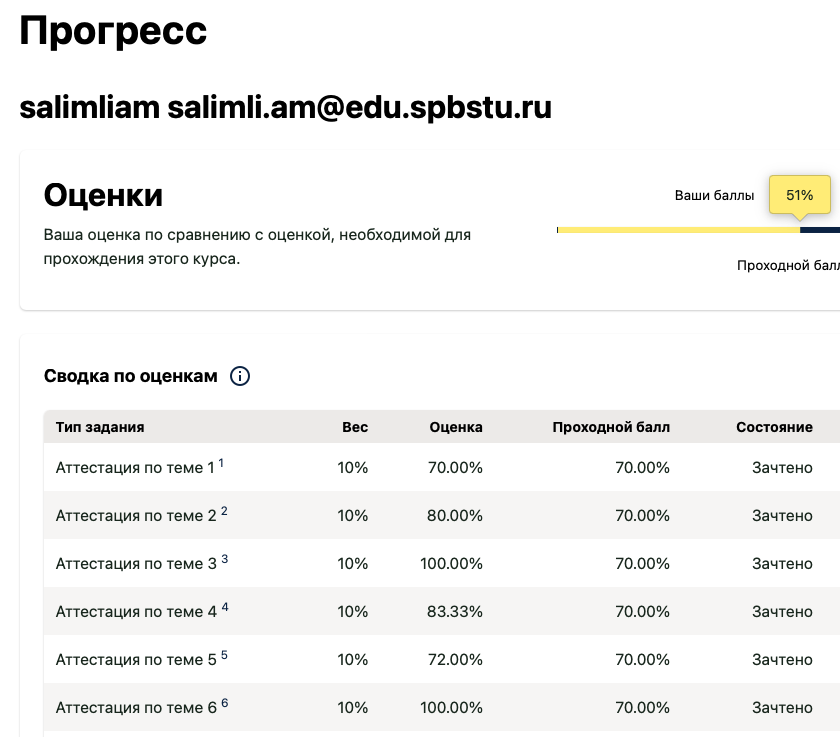
\includegraphics[width=0.8\textwidth]{images/111.png}
    \caption{Прогресс}
    \label{fig:1}
\end{figure}

\begin{figure}[H]
    \centering
    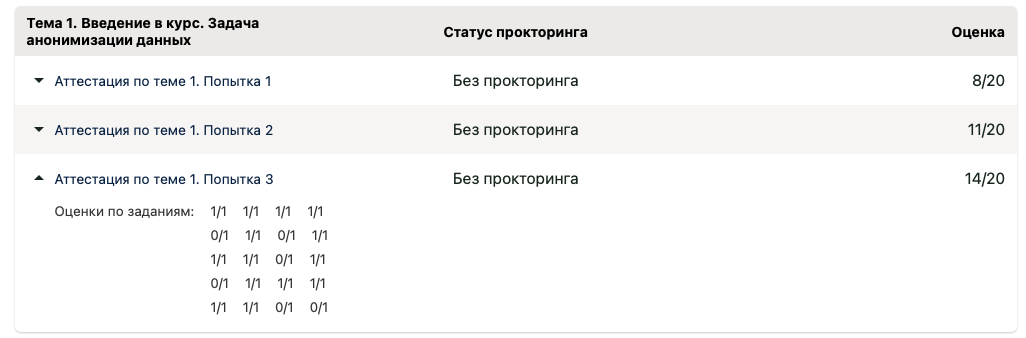
\includegraphics[width=0.8\textwidth]{images/1.png}
    \caption{Результаты прохождения аттестации по теме 1}
    \label{fig:2}
\end{figure}

\begin{figure}[H]
    \centering
    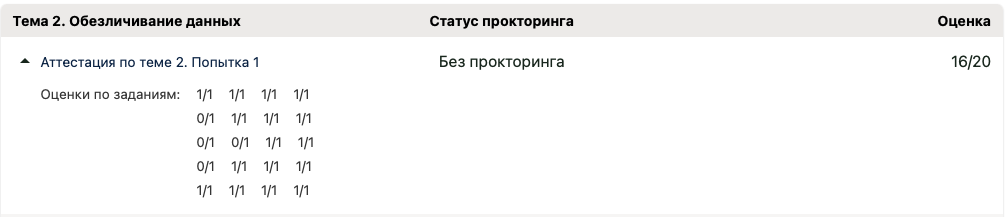
\includegraphics[width=0.8\textwidth]{images/2.png}
    \caption{Результаты прохождения аттестации по теме 2}
    \label{fig:3}
\end{figure}

\begin{figure}[H]
    \centering
    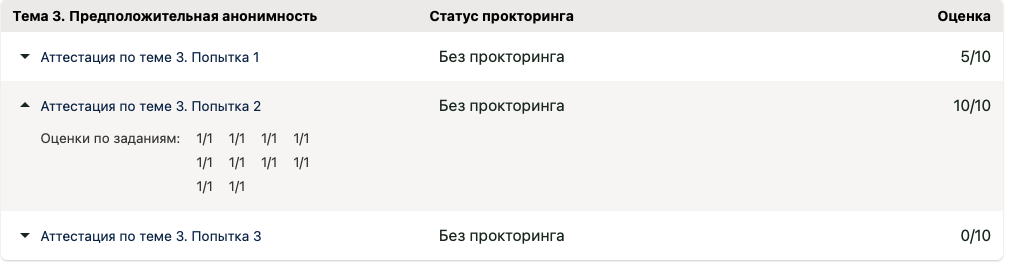
\includegraphics[width=0.8\textwidth]{images/3.png}
    \caption{Результаты прохождения аттестации по теме 3}
    \label{fig:4}
\end{figure}               

\begin{figure}[H]
    \centering
    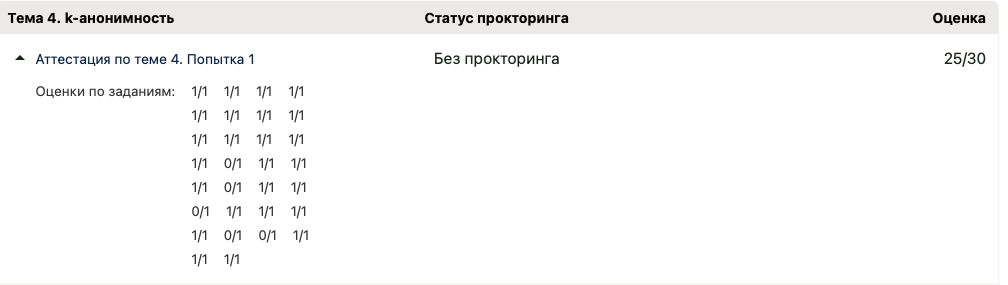
\includegraphics[width=0.8\textwidth]{images/4.png}
    \caption{Результаты прохождения аттестации по теме 4}
    \label{fig:5}
\end{figure}

\begin{figure}[H]
    \centering
    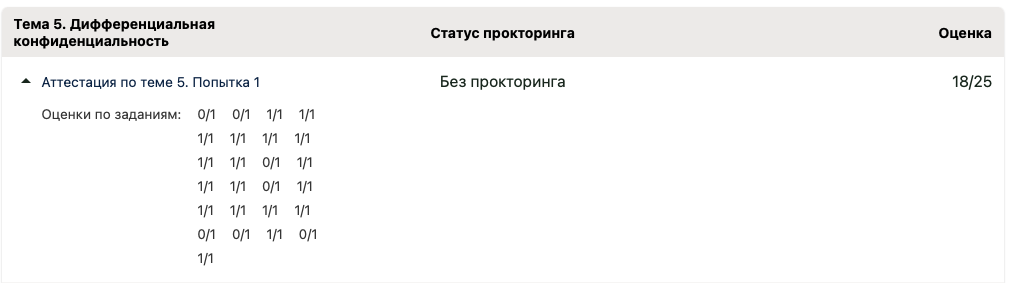
\includegraphics[width=0.8\textwidth]{images/5.png}
    \caption{Результаты прохождения аттестации по теме 5}
    \label{fig:6}
\end{figure}   

\begin{figure}[H]
    \centering
    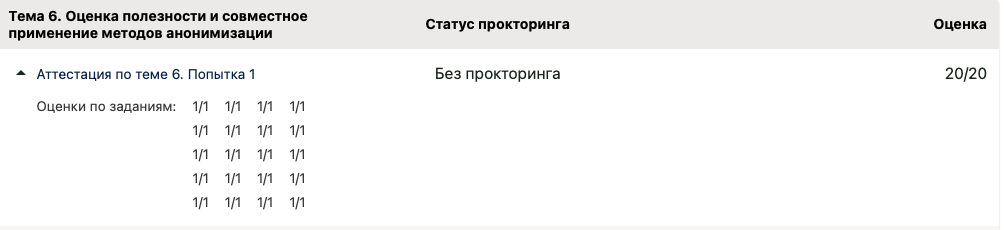
\includegraphics[width=0.8\textwidth]{images/6.png}
    \caption{Результаты прохождения аттестации по теме 6}
    \label{fig:7}
\end{figure}
\newpage
\section{Заключение}
Прохождение онлайн-курса «Анонимизация данных», автором которого является Полтавцева Мария Анатольевна, позволило ознакомиться с фундаментальными концепциями и принципами современных методов защиты персональных данных. Курс охватывал широкий спектр тем, включая основы анонимизации и обезличивания данных, методы защиты от атак идентификации, а также практические аспекты реализации механизмов конфиденциальности в информационных системах. Одной из ключевых особенностей курса стала связь изучаемых технологий с актуальными требованиями законодательства в области защиты персональных данных.
Курс предоставил глубокое понимание роли современных методов анонимизации в обеспечении баланса между доступностью данных для анализа и сохранением конфиденциальности персональной информации. Особенно ценным оказалось изучение таких концепций как k-анонимность и дифференциальная конфиденциальность, которые являются основой современных подходов к защите данных.
Подводя итоги, хочется отметить, что использование дистанционных образовательных технологий, на которых базировался данный курс, представляет собой важное дополнение к традиционным методам обучения. Однако, несмотря на очевидные преимущества онлайн-обучения, такие как гибкость и доступность, личное общение с преподавателем и участие в практических занятиях остаются незаменимыми для полноценного усвоения материала, особенно в области, требующей практического применения различных методов анонимизации.
Онлайн-курсы, подобные этому, играют важную роль в расширении образовательных возможностей и развитии самостоятельного обучения. Они отлично дополняют основное образование, предоставляя удобные инструменты для освоения сложных концепций и навыков, востребованных в современных системах защиты информации.
\newpage
\section{Список источников}
\begin{enumerate}
    \item Анонимизация данных. Открытое образование: URL: \url{https://apps.openedu.ru/learning/course/course-v1:spbstu+DATANON+spring_2025/progress}(дата обращения: 15.05.2025)
\end{enumerate}
\end{document}